\ifx\XeTeXversion\undefined\pdfoutput=1\pdfminorversion=7\fi
\documentclass[10pt,twocolumn,letterpaper]{article}

\usepackage[top=0.80in,bottom=0.82in,left=0.70in,right=0.70in,columnsep=0.25in]{geometry}
\usepackage{amsmath,amssymb,bm}
\usepackage{booktabs}
\usepackage{graphicx}
\usepackage{xcolor}
\usepackage[font=small,labelfont=bf]{caption}
\usepackage{microtype}
\usepackage[hidelinks]{hyperref}
\usepackage{url}

\ifx\XeTeXversion\undefined
  \usepackage[utf8]{inputenc}
  \usepackage[T1]{fontenc}
  \usepackage{lmodern}
  \usepackage{CJKutf8}
  \newcommand{\zh}[1]{\begin{CJK*}{UTF8}{gbsn}{\small #1}\end{CJK*}}
\else
  \usepackage{fontspec}
  \usepackage{xeCJK}
  \setCJKmainfont[Scale=0.90]{Songti SC}
  \newcommand{\zh}[1]{#1}
\fi

% Crisp two-column academic heading hierarchy (matching ACL/NeurIPS proportions without external packages)
\makeatletter
\renewcommand\section{\@startsection {section}{1}{\z@}%
  {-2.2ex \@plus -0.6ex \@minus -0.2ex}%
  {1.0ex \@plus 0.2ex}%
  {\normalfont\large\bfseries\raggedright}}
\renewcommand\subsection{\@startsection{subsection}{2}{\z@}%
  {-1.8ex \@plus -0.4ex \@minus -0.2ex}%
  {0.7ex \@plus 0.15ex}%
  {\normalfont\normalsize\fontsize{10.8}{13}\selectfont\bfseries\raggedright}}
\renewcommand\subsubsection{\@startsection{subsubsection}{3}{\z@}%
  {-1.4ex \@plus -0.3ex \@minus -0.1ex}%
  {0.5ex \@plus 0.1ex}%
  {\normalfont\normalsize\bfseries\itshape\raggedright}}
\makeatother

\definecolor{crimson}{HTML}{BE123C}
\definecolor{tealaccent}{HTML}{0F4C5C}
\definecolor{slatebg}{HTML}{F8FAFC}
\definecolor{slateborder}{HTML}{CBD5E1}

\newcommand{\propbox}[2]{%
  \par\medskip\noindent
  \fcolorbox{slateborder}{slatebg}{%
    \parbox{\dimexpr\columnwidth-2\fboxsep-2\fboxrule\relax}{%
      \textbf{#1.}\ \emph{#2}%
    }%
  }\par\medskip
}

\setlength{\parskip}{2pt}
\setlength{\emergencystretch}{1.5em}
\renewcommand{\UrlFont}{\ttfamily\small}

\title{\textbf{Chime: Sub-3ms On-Device Neural Pinyin Input\\via Manifold-Aligned Distillation and Rank-Stacked Multi-LoRA Cartridges}}

\author{
  \textbf{Tian Chen}\\
  {\small Independent Systems \& Machine Learning Research $\cdot$ \texttt{tyr.chen@gmail.com} $\cdot$ \url{https://github.com/tyrchen/chime}}
}
\date{}

\begin{document}

\twocolumn[{%
  \maketitle
  \vspace{-1.2em}
  \begin{center}
  \fcolorbox{slateborder}{slatebg}{%
    \parbox{0.93\textwidth}{%
      \vspace{2pt}
      \begin{center}\textbf{Abstract}\end{center}
      \vspace{-4pt}
      {\small
      Applying Large Language Models (LLMs) to client-side Pinyin Input Method Editors (IMEs) faces a strict systems trilemma: human typing demands sub-10\,ms keystroke latency without candidate-bar jitter, operating systems enforce tight resident memory budgets ($< 100$\,MB) alongside zero-network privacy guarantees, and real-world input spans open-domain vocabulary from bilingual code identifiers to classical literature and idiosyncratic personal style. Existing generative Pinyin-to-Character (P2C) LLMs violate latency budgets via autoregressive decoding and suffer catastrophic representation collapse under aggressive layer pruning or out-of-vocabulary (OOV) blindness when relying solely on parameter-efficient adapters. We present \textbf{Chime}, a 100\% offline neural IME for Apple Silicon that resolves this trilemma through lexical-neural co-design. First, we formalize \emph{Recall--Rerank Decoupling} and \emph{Probability-Space Separation}, pairing a $< 0.8$\,ms zero-copy \texttt{mmap} dual-track lattice decoder (\texttt{CHIMED02}) with a batched prefix-cached causal language model reranker that isolates equal-span homophone scoring from variable-horizon lookahead completions. Second, we compress the 28-layer \texttt{Qwen3-0.6B} (1.19\,GB FP16) into a 6-layer, 24,576-vocab 4-bit MLX student (\textbf{64.17\,MB}, $18.6\times$ smaller); whereas naive layer skipping collapses pre-head teacher alignment to $\cos(\bm{u}_S, \bm{u}_T) = 0.022$ and halves homophone accuracy to 43.8\%, our \emph{Manifold-Aligned Layer Distillation} restores $\cos(\bm{u}_S, \bm{u}_T) = 0.853$, matching the 28-layer teacher's \textbf{93.8\%} (15/16) zero-shot stress accuracy and achieving \textbf{100\%} (44/44) end-to-end IME accuracy at \textbf{0.86\,ms} 6-candidate Metal reranking latency ($6.15\times$ faster than 28-layer 4-bit). Third, we introduce pluggable \emph{\texttt{.imepack} cartridges} that co-mount zero-copy lexical slices (\texttt{pack.imedict}) with \emph{Q4-Manifold Aligned} 2.07\,MB Rank-8 \texttt{LoRA} sidecars. Combining \emph{Rank-Stacked GEMM Fusion}, \emph{Batched Broadcast KV-Gather}, and a \emph{Couplet-Aware Simplex Router} cuts 6-adapter reranking latency from 10.82\,ms to \textbf{1.45\,ms} (\textbf{$7.46\times$ speedup}, $+39.6\,\mu\text{s}$/adapter), eliminates multi-adapter register drift, and removes FP16$\to$INT4 scale overshoot ($-0.270$\,nats classical NLL gain).
      \par}
      \vspace{2pt}
    }%
  }
  \end{center}
  \vspace{0.8em}
}]

\section{Introduction}

Every sentence written on a desktop or mobile device passes through an Input Method Editor (IME). For over a billion Chinese speakers, Pinyin-to-Character (P2C) conversion is a quintessential noisy-channel inference problem~\cite{chen2000new,jia2014joint}: a user types a romanized phonetic keystroke stream---frequently interleaved with initial-letter abbreviations (\texttt{wsm} $\to$ \zh{为什么}), regional phonetic mergers (\texttt{z}/\texttt{zh}, \texttt{in}/\texttt{ing}), motor slips on QWERTY layouts (\texttt{shaung} $\to$ \texttt{shuang}), and unswitched English identifiers (\texttt{macOS}, \texttt{GitHub})---expecting the intended text at slot \#1 within a single display frame.

Recent advances in Large Language Models (LLMs) have inspired a wave of generative IME prototypes~\cite{tan2022exploring,ding2023geneinput,gui2025attninput,shan2026huoziime} that cast P2C as end-to-end conditional sequence generation. Despite strong perplexity on clean benchmarks, deploying LLMs inside a production OS input method exposes a fundamental \textbf{Latency--Memory--Recall Trilemma}:
\begin{enumerate}
  \item \textbf{Perceptual Latency \& Visual Jitter}: Human typists perceive interface lag above 10--15\,ms and commit muscle-memory errors if slot \#1 shifts after $\approx 60$\,ms of visual fixation. Autoregressive LLM generation over candidate character sequences incurs 25--150\,ms per keystroke even on modern accelerators, while cloud-offloaded IMEs introduce variable network tail latency and transmit every keystroke off-device.
  \item \textbf{Resident Memory Ceiling \& Collapse}: An OS-resident background service active across every window cannot consume gigabytes of RAM. Yet naively pruning a 28-layer, 1.19\,GB model (\texttt{Qwen3-0.6B}~\cite{yang2025qwen3}) down to 6 layers and 4-bit weights ($\approx 64$\,MB) destroys the alignment between intermediate transformer blocks and the frozen vocabulary embedding head, collapsing cosine similarity to $0.022$ and degrading homophone disambiguation to near-chance (43.8\%).
  \item \textbf{Lexical Recall vs.\ Multi-Domain Interference}: Neither a 64\,MB base model nor Low-Rank Adaptation (\texttt{LoRA}~\cite{hu2022lora}) alone can recall 260,000+ long-tail classical verses (e.g., \zh{念去去，千里烟波}) if Stage-1 beam search prunes them. Conversely, mounting multiple domain \texttt{LoRA}s simultaneously (e.g., classical literature, developer prose, and personal essays) triggers two failure modes on edge GPUs: \emph{Register Superposition Drift}---where summing written-domain adapters overwhelms colloquial priors (flipping \zh{究竟有多大} to \zh{多达})---and \emph{Sequential Kernel Launch Inflation}, which scales latency linearly with adapter count $K$.
\end{enumerate}

\begin{figure*}[t]
  \centering
  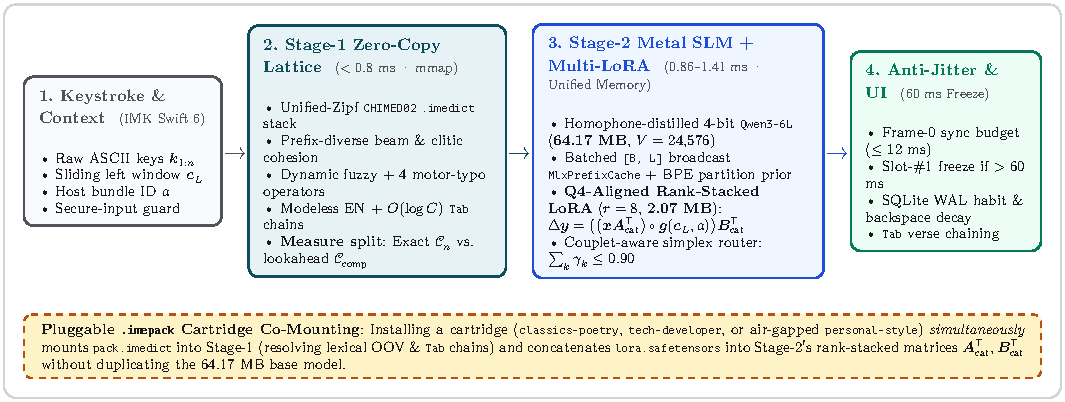
\includegraphics[width=\textwidth]{fig1_architecture.pdf}
  \vspace{-1.2em}
  \caption{End-to-end architecture of \textbf{Chime}. Stage~1 maps layered \texttt{CHIMED02} binary dictionaries via \texttt{mmap} ($< 0.8$\,ms) and separates equal-span candidates $\mathcal{C}_n$ from lookahead completions $\mathcal{C}_{\text{comp}}$. Stage~2 runs a frozen 64.17\,MB 4-bit \texttt{Qwen3-6L} student with batched broadcast \texttt{MlxPrefixCache}, on-GPU \texttt{take\_along\_axis}, and fused Rank-Stacked \texttt{.imepack} \texttt{LoRA} sidecars under a 60\,ms anti-jitter contract.}
  \label{fig:arch}
\end{figure*}

In this paper, we design, implement, and empirically evaluate \textbf{Chime}, an open-source, zero-telemetry macOS IME written in Rust and Swift~6 on Apple Silicon Unified Memory~\cite{hannun2023mlx}. Rather than forcing a compact LLM to hallucinate character mappings from raw keystrokes, Chime establishes a principled division of labor between deterministic zero-copy data structures and manifold-aligned low-rank neural rescoring (Figure~\ref{fig:arch}). Our primary contributions are fourfold:
\begin{itemize}
  \item \textbf{Recall--Rerank Co-Design \& Measure Separation (\S\ref{sec:formulation})}: We prove that Stage-2 neural rescoring is upper-bounded by Stage-1 pool recall and must separate equal-span homophone hypotheses $\mathcal{C}_n$ from lookahead completions $\mathcal{C}_{\text{comp}}$ to avoid cross-horizon probability distortion, paired with sublinear length calibration $|c|^{-0.42}$ across heterogeneous BPE tokenizations.
  \item \textbf{Manifold-Aligned 6-Layer Student Distillation (\S\ref{sec:distill})}: Combining vocabulary pruning ($151{,}936 \to 24{,}576$ tokens), frozen tied embeddings, trajectory MSE, pre-head cosine alignment, and dual-temperature KL distillation, we compress \texttt{Qwen3-0.6B} by $18.6\times$ into a 64.17\,MB 4-bit MLX student that matches the 28-layer teacher's zero-shot disambiguation accuracy (93.8\%) at \textbf{0.86\,ms} 6-candidate batched reranking ($6.15\times$ faster).
  \item \textbf{Rank-Stacked \texttt{.imepack} Cartridges \& Q4-Manifold Alignment (\S\ref{sec:lora})}: We package zero-copy \texttt{pack.imedict} slices alongside 2.07\,MB Rank-8 \texttt{LoRA}s into hot-swappable cartridges. Combining \emph{Rank-Stacked GEMM Fusion} with \emph{Batched Broadcast KV-Gather} (\texttt{take\_along\_axis}) cuts 6-adapter reranking from 10.82\,ms to \textbf{1.45\,ms} (\textbf{$7.46\times$ speedup}, $+39.6\,\mu\text{s}$ marginal cost/adapter), while \emph{Q4-Manifold LoRA Training} and our \emph{Couplet-Aware Simplex Router} eliminate multi-adapter register drift and INT4 transfer overshoot.
  \item \textbf{System Evaluation \& Longitudinal Personalization (\S\ref{sec:exp})}: Across classical Chinese (266K entries, 231K \texttt{Tab} chains), developer code-switching, and an air-gapped 815K-character pre-LLM longitudinal personal corpus (2013--2020), Chime achieves \textbf{44/44 (100\%)} benchmark accuracy and $9\times$ classical recall gain ($10.0\% \to 90.0\%$).
\end{itemize}

\section{Related Work}

\textbf{Statistical and Graph-Based Pinyin Decoding.} Classical P2C engines model conversion as Viterbi search over word lattices weighted by character/word \mbox{$n$-grams}~\cite{chen2000new} and double-array tries~\cite{yoshinaga1992double}. Jia and Zhao~\cite{jia2014joint} introduced a joint graph model integrating QWERTY typo correction with P2C conversion. While sub-millisecond and memory-frugal, finite-context \mbox{$n$-grams} fail on context-sensitive homophones (e.g., \zh{保障}\textbf{\zh{权利}} [safeguard rights] vs.\ \zh{滥用}\textbf{\zh{权力}} [abuse power], especially across intervening modifiers).

\textbf{Neural and LLM-Based Input Methods.} Zhang et~al.~\cite{zhang2019open} augmented neural P2C with online open-vocabulary sampling. Xu et~al.~\cite{xu2022pert} proposed \texttt{PERT}, a bidirectional encoder pre-trained directly on Pinyin sequences. With the rise of generative LLMs, Tan et~al.~\cite{tan2022exploring} adapted frozen Chinese GPT to P2C, observing severe degradation on abbreviated Pinyin due to combinatorial candidate explosion. \texttt{GeneInput}~\cite{ding2023geneinput} unified full-mode key-to-character generation via prompting and RLHF, \texttt{AttnInput}~\cite{gui2025attninput} attached a Pinyin side-network to linear RWKV models, and \texttt{HuoziIME}~\cite{shan2026huoziime} explored on-device LLM personalization via hierarchical memory. Unlike these end-to-end generative designs---which struggle with sub-5\,ms keystroke budgets, multi-syllable typo graphs, and exact casing for code-switching---Chime retains deterministic $O(\log N)$ lattice recall in Stage~1 and deploys a prefix-cached causal SLM strictly as a constant-depth parallel rescorer in Stage~2.

\textbf{Edge Compression and Multi-LoRA Serving.} Knowledge distillation~\cite{hinton2015distilling} with hidden-state alignment (\texttt{TinyBERT}~\cite{jiao2020tinybert}) and group-wise weight quantization (\texttt{GPTQ}~\cite{frantar2023gptq}, \texttt{AWQ}~\cite{lin2024awq}) enable compact edge deployment. In cloud serving, \texttt{S-LoRA}~\cite{sheng2024slora} batches heterogeneous requests across per-tenant adapters using paging kernels, whereas personalized \texttt{LoRA} routing (\texttt{PLoRA}~\cite{zhang2024plora}) blends adapters per user. To our knowledge, Chime is the first system to investigate \emph{single-stream concurrent Multi-LoRA superposition} on unified-memory client GPUs---identifying and solving both multi-adapter register interference and FP16-to-INT4 manifold shift.

\section{Problem Formulation \& Hybrid Co-Design}\label{sec:formulation}

\subsection{Joint Phonetic-Typo-Code Lattice Decoding}

Given a raw ASCII keystroke sequence $\bm{k} = k_{1:n}$, surrounding left document context $\bm{c}_L$ (bounded to 96 characters), and active host application identifier $a$ (e.g., \texttt{com.mitchellh.ghostty} vs.\ \texttt{md.obsidian}), an IME seeks the highest-scoring surface string $\bm{w}^*$:
\begin{equation}\label{eq:joint}
\begin{aligned}
  \bm{w}^* = \arg\max_{\bm{w} \in \mathcal{G}(\bm{k})} \Big[ & S_{\text{lex}}(\bm{w}, \bm{k} \mid \bm{c}_L, a) \\
  & + \lambda \cdot S_{\text{slm}}(\bm{w} \mid \bm{c}_L, a) \Big]
\end{aligned}
\end{equation}
where $\mathcal{G}(\bm{k})$ is the dual-track segmentation lattice constructed over byte spans $[i, j) \subseteq [0, n)$.

To achieve $< 0.8$\,ms Stage-1 construction without memory bloat, Chime compiles static and cartridge lexicons into \texttt{CHIMED02}, a 48-byte-header immutable binary image mapped directly into virtual memory via \texttt{mmap} (\texttt{memmap2}). Rather than expanding fuzzy Pinyin permutations offline---which multiplies dictionary size by $2^6$---Stage~1 evaluates an algebraic equivalence relation $\mathcal{F}(s)$ (\texttt{z}$\leftrightarrow$\texttt{zh}, \texttt{an}$\leftrightarrow$\texttt{ang}, \texttt{in}$\leftrightarrow$\texttt{ing}, etc.) dynamically at span-lookup time, alongside four 1-edit motor-noise operators on raw slice $\bm{k}_{i:j}$:
\begin{enumerate}
  \item \emph{Adjacent transposition} (\texttt{shaung} $\to$ \texttt{shuang}, \texttt{uq} $\to$ \texttt{qu}, cost $\delta_{\text{swap}} = 1.05$);
  \item \emph{QWERTY Euclidean neighbor substitution} ($d^2 \le 1.85$ key pitches, e.g., \texttt{shuruga} $\to$ \texttt{shurufa}, cost $0.85 + 0.45 d^2$);
  \item \emph{Accidental key-repeat deletion} (\texttt{niian} $\to$ \texttt{nian}, cost $\delta_{\text{rep}} = 1.10$);
  \item \emph{Geminate boundary consonant elision} (\texttt{chunuan} $\to$ \texttt{chun}+\texttt{nuan} \zh{春暖}, \texttt{jiangun} $\to$ \texttt{jiang}+\texttt{gun} \zh{江滚} when a shared coda/onset \texttt{n} or \texttt{g} is pressed once before a vowel, cost $\delta_{\text{gem}} = 0.85$).
\end{enumerate}

Multi-syllable exact phrases, idioms, and merged classical clauses up to 16 syllables are traversed via depth-first span expansion gated at every step by an $O(\log N)$ binary search (\texttt{has\_longer\_pinyin\_prefix}) over sorted 16-byte \texttt{pinyin\_groups}, pruning dead typo branches immediately at length 1--2. Simultaneously, a parallel code-switching track scores canonical-case English identifiers (\texttt{macos} $\to$ \texttt{macOS}, \texttt{chatgpt} $\to$ \texttt{ChatGPT}) and camelCase tokens (\texttt{useEffect}) with automatic Pangu boundary spacing.

\subsection{Recall--Rerank Decoupling \& Measure Separation}

Why not rely on \texttt{LoRA} fine-tuning alone to inject domain phrases or classical poetry? Let $\mathcal{C}_M(\bm{k}) \subset \mathcal{G}(\bm{k})$ denote the top-$M$ candidates retained by Stage-1 beam search ($M=15$).

\propbox{Proposition 1 (Stage-1 Recall Bottleneck)}{For any finite Stage-2 rescorer $S_{\text{slm}} : \Sigma^* \to \mathbb{R}$ with bounded dynamic range $|S_{\text{slm}}| \le B$, if a target multi-character entity or verse $\bm{w}^*$ is absent from the mounted lexicon such that fragmented character paths push $\bm{w}^*$ outside $\mathcal{C}_M(\bm{k})$, then $\mathbb{P}(\bm{w}^* = \bm{w}_1) = 0$ regardless of \texttt{LoRA} rank $r$ or Stage-2 capacity.}

Proposition~1 explains why typing \texttt{mingyuejishiyou} without a classical lexicon yields \zh{明月即使有} (\emph{``even if the bright moon...''}): modern high-frequency bigrams (\zh{即使}, $\log P = -3.8$) dominate fragmented character beams (\zh{几} + \zh{时}, $\log P = -8.9$), evicting \zh{明月几时有} before Stage~2 executes.

Equally critical is \emph{which} candidates inside $\mathcal{C}_M(\bm{k})$ may be compared by $S_{\text{slm}}$. Modern IMEs surface both \emph{full-span interpretations} $\mathcal{C}_n$ (consuming $\bm{k}_{1:n}$) and \emph{prefix lookahead completions} $\mathcal{C}_{\text{comp}}$ (e.g., typing 3 syllables \texttt{junbujian} surfaces the 10-syllable verse completion \zh{君不见高堂明镜悲白发}).

\propbox{Proposition 2 (Measure Incompatibility across Horizons)}{Let $\bm{w}_s \in \mathcal{V}^m$ be an $m$-character full-span candidate and $\bm{w}_\ell = \bm{w}_s \circ \bm{w}_{\text{rem}} \in \mathcal{V}^{m+d}$ ($d \ge 1$) be a lookahead completion extending $\bm{w}_s$. Under any causal language model $P_\theta$, by the chain rule, $\log P_\theta(\bm{w}_\ell \mid \bm{c}_L) = \log P_\theta(\bm{w}_s \mid \bm{c}_L) + \sum_{t=1}^d \log P_\theta(w_{m+t} \mid \bm{c}_L, \bm{w}_{<m+t}) < \log P_\theta(\bm{w}_s \mid \bm{c}_L)$ whenever $P_\theta(w_{m+t} \mid \cdot) < 1$. Under sublinear length normalization $|\bm{w}|^\alpha$ ($\alpha < 1$), $\bm{w}_\ell$ incurs a systematic horizon penalty of $\Theta(d^{1-\alpha})$ nats relative to $\bm{w}_s$.}

Guided by Proposition~2, Chime enforces \emph{Probability-Space Separation}: Stage-2 zero-meaned neural rescoring operates strictly over the equal-input homophone subspace $\mathcal{C}_n \setminus \mathcal{C}_{\text{comp}}$, while lookahead completions $\mathcal{C}_{\text{comp}}$ are governed by prefix selectivity and deterministic $O(\log C)$ continuation chains (\texttt{continuations\_off} at byte offset 40 of \texttt{CHIMED02}), plus an anti-repeat penalty ($-5.5$\,nats) if a \mbox{$\ge 5$-character} verse already appears in $\bm{c}_L$.

Within $\mathcal{C}_n \setminus \mathcal{C}_{\text{comp}}$, candidates share identical character length ($|\bm{w}|$) on homophones (\zh{权利} vs.\ \zh{权力}) yet often differ in BPE token count $T(\bm{w})$: formal compounds like \zh{多达} occupy 1 subword token, whereas colloquial phrases like \zh{多大} split into 2 tokens (\zh{多} + \zh{大}). Dividing by $T(\bm{w})$ artificially inflates 2-token candidates because splitting a joint probability $\log P(w_1, w_2)$ by 2 halves its magnitude; instead, Chime sums the \emph{exact unnormalized joint log-likelihood} $\ell(\bm{w}) = \sum_{t=1}^{T(\bm{w})} \log P_\theta(z_t \mid \bm{c}_L, z_{<t})$ and normalizes solely by \emph{character length} $|\bm{w}|^{0.42}$:
\begin{equation}\label{eq:rerank}
  S_{\text{slm}}(\bm{w} \mid \bm{c}_L, a) = \lambda \left( \frac{\ell(\bm{w})}{|\bm{w}|^{0.42}} - \frac{1}{|\mathcal{B}|} \sum_{\bm{w}' \in \mathcal{B}} \frac{\ell(\bm{w}')}{|\bm{w}'|^{0.42}} \right)
\end{equation}
where $\lambda = 0.65$ and $\mathcal{B} \subseteq \mathcal{C}_n \setminus \mathcal{C}_{\text{comp}}$ ($|\mathcal{B}| \le 6$).

\section{Manifold-Aligned 6-Layer Distillation}\label{sec:distill}

\subsection{Vocabulary Pruning \& Naive Skip Collapse}

Our teacher is \texttt{Qwen/Qwen3-0.6B-Base}~\cite{yang2025qwen3} ($L_T = 28$ layers, $d = 1024$, $d_{\text{ff}} = 3072$, 16 query heads, 8 KV heads with \texttt{head\_dim} $= 128$, QK-RMSNorm, tied embeddings, and vocabulary $V_T = 151{,}936$, totaling 1,191.5\,MB in FP16). In a 6-layer student with full vocabulary, the $151{,}936 \times 1024$ embedding table alone consumes 311\,MB in FP16 (78\,MB in 4-bit), dominating the transformer blocks. We prune the vocabulary to $V_S = 24{,}576$ pieces covering all GB2312/common Unihan characters, high-frequency Chinese multi-character subwords, punctuation, and ASCII/developer subwords, shrinking the 4-bit embedding table by \textbf{83.8\%} to \textbf{12.6\,MB}.

However, initializing a 6-layer student by uniformly selecting teacher layers $\mathcal{I} = \{0, 5, 11, 16, 22, 27\}$ while freezing the pruned teacher embedding matrix $\bm{E} \in \mathbb{R}^{V_S \times d}$ causes severe \emph{Manifold Misalignment}. Because residual transformers refine representations incrementally across 28 blocks before projecting onto $\bm{E}^\top$, skipping 22 blocks rotates the pre-head hidden vector $\bm{u}_S = \text{RMSNorm}(\bm{h}_S^{(6)})$ nearly orthogonal to the teacher's $\bm{u}_T = \text{RMSNorm}(\bm{h}_T^{(28)})$: empirically, $\cos(\bm{u}_S, \bm{u}_T)$ plummets to \textbf{0.0221} (Table~\ref{tab:pareto}), causing colloquial \zh{多大} to lose to \zh{多达} and cutting homophone accuracy to 43.8\%.

\subsection{Composite Trajectory \& Cosine-KL Objective}

To realign the 6-layer student directly onto the frozen teacher embedding geometry $\bm{E}$ (preventing embedding overfitting on finite distillation corpora), we freeze $\bm{E}$ and optimize only the 6 transformer blocks $\theta_S$ over 9.94M tokens of mixed conversational, encyclopedic, code-switching, and literary text using a three-term objective:
\begin{equation}\label{eq:distill}
\begin{aligned}
  \mathcal{L}(\theta_S) &= \alpha_{\text{kl}} \mathcal{L}_{\text{DKL}} + \alpha_{\text{cos}} \big(1 - \cos(\bm{u}_S, \bm{u}_T)\big) \\
  &\quad + \frac{\alpha_{\text{hid}}}{|\mathcal{M}|} \sum_{(m, \ell) \in \mathcal{M}} \big\| \hat{\bm{h}}_S^{(m)} - \hat{\bm{h}}_T^{(\ell)} \big\|_2^2
\end{aligned}
\end{equation}
where $\hat{\bm{h}} = \bm{h} / \|\bm{h}\|_2$ aligns intermediate block trajectories across layer map $\mathcal{M} = \{(1,5), (2,11), (3,16), (4,22), (5,27)\}$, and $\mathcal{L}_{\text{DKL}}$ is a \emph{Dual-Temperature Forward KL} over the pruned 24,576-logit head $\bm{z} = \bm{u} \bm{E}^\top$:
\begin{equation}\label{eq:dkl}
\begin{aligned}
  \mathcal{L}_{\text{DKL}} &= 0.7 \tau_1^2 D_{\text{KL}}\!\big(\sigma(\bm{z}_T / \tau_1) \,\|\, \sigma(\bm{z}_S / \tau_1)\big) \\
  &\quad + 0.3 D_{\text{KL}}\!\big(\sigma(\bm{z}_T) \,\|\, \sigma(\bm{z}_S)\big)
\end{aligned}
\end{equation}
with $\tau_1 = 2.0$, $\alpha_{\text{kl}} = 1.0$, $\alpha_{\text{cos}} = 2.5$, and $\alpha_{\text{hid}} = 1.5$. Training for 1,600 steps (batch 32, length 192, peak LR $3 \times 10^{-4}$) on a single NVIDIA L4 GPU takes 14 minutes, driving $\cos(\bm{u}_S, \bm{u}_T)$ from $0.0221 \to 0.9310$ on validation sequences ($0.8531$ after group-64 4-bit MLX affine quantization into \textbf{64.17\,MB}).

\section{Rank-Stacked Multi-LoRA Cartridges}\label{sec:lora}

\subsection{The \texttt{.imepack} Cartridge Abstraction}

To let users extend Chime across specialized domains without bloating or retraining the 64.17\,MB base model, we introduce \texttt{.imepack} v2 cartridges. Each cartridge bundles:
(1)~\texttt{pack.imedict}: a zero-copy \texttt{CHIMED02} slice containing domain words, canonical English terms, \mbox{$n$-grams}, and $O(\log C)$ \texttt{Tab} continuation records;
(2)~\texttt{lora.safetensors}: Rank-$r$ ($r=8$) FP16 low-rank matrices $(\bm{A}_k^{(\ell, p)} \in \mathbb{R}^{r \times d_{\text{in}}}, \bm{B}_k^{(\ell, p)} \in \mathbb{R}^{d_{\text{out}} \times r})$ across all 7 linear projections $p \in \{q, k, v, o, \text{gate}, \text{up}, \text{down}\}$ of all 6 layers ($1{,}032{,}192$ parameters $= 2.07$\,MB per pack); and
(3)~\texttt{manifest.json}: declaring routing policy (\texttt{classical}, \texttt{developer}, or \texttt{always}), base scale $s_k$, and privacy flag \texttt{private\_pack}.

\begin{figure*}[t]
  \centering
  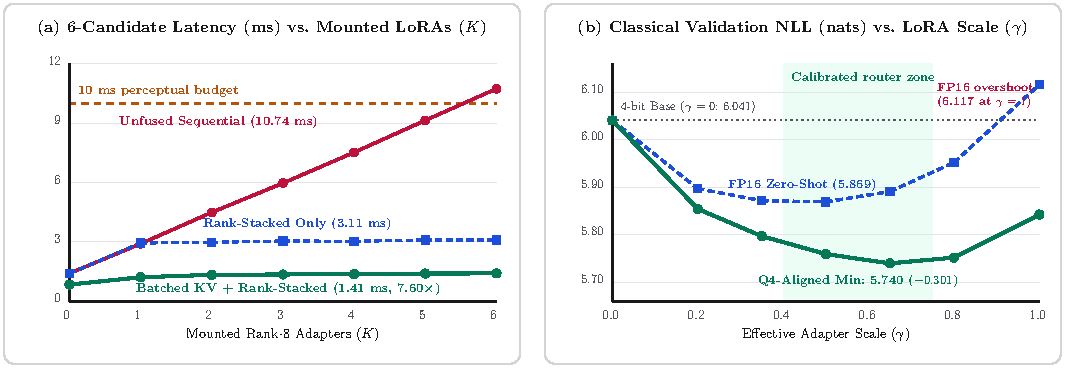
\includegraphics[width=\textwidth]{fig2_scaling.pdf}
  \vspace{-1.2em}
  \caption{\textbf{(a)} Measured 6-candidate Metal reranking latency (p50, ms) across $K = 0, \dots, 6$ Rank-8 cartridges: Rank-Stacked GEMMs flatten the $O(K)$ kernel ramp ($10.82 \to 3.29$\,ms), and Batched Broadcast KV-Gather cuts it further to \textbf{0.87\,ms} ($K=0$) and \textbf{1.45\,ms} ($K=6$, \textbf{$7.46\times$ speedup}). \textbf{(b)} Classical validation NLL vs.\ adapter scale $\gamma$: zero-shot transfer of an FP16-trained LoRA overshoots at $\gamma = 1.0$ (6.071), whereas \textbf{Q4-Manifold Aligned LoRA} training directly on dequantized 4-bit weights eliminates overshoot and deepens NLL reduction by 68\% ($5.978 \to \mathbf{5.708}$).}
  \label{fig:scaling}
\end{figure*}

\subsection{Rank-Stacked GEMM Fusion \& Batched KV-Gather}

When $K$ cartridges are mounted concurrently, a naive implementation evaluates each active adapter sequentially inside every linear layer:
\begin{equation}\label{eq:unfused}
  \bm{y} = \text{QuantMatmul}_{\text{4bit}}(\bm{x}, \widehat{\bm{W}}) + \sum_{k=1}^K \gamma_k (\bm{x} \bm{A}_k^\top) \bm{B}_k^\top
\end{equation}
Across 6 layers and 7 projections, Eq.~\eqref{eq:unfused} dispatches $42 \times 2K$ tiny skinny-matrix multiplications plus $42 \times 2K$ scalar/add kernels per forward pass, causing 6-candidate reranking latency to grow linearly by $+1.58$\,ms per adapter to 10.82\,ms at $K=6$ (Figure~\ref{fig:scaling}a).

We eliminate this bottleneck via two complementary GPU optimizations:
\begin{enumerate}
  \item \textbf{Rank-Stacked GEMM Fusion}: At cartridge mount time, Chime pre-transposes and concatenates all $K$ adapters along the rank dimension once in Unified Memory ($R = \sum_{k=1}^K r_k = 8K$):
  \begin{equation}\label{eq:stacked}
  \begin{aligned}
    \bm{A}_{\text{cat}}^\top &= [\bm{A}_1^\top \cdots \bm{A}_K^\top] \in \mathbb{R}^{d_{\text{in}} \times R}, \\
    \bm{B}_{\text{cat}}^\top &= [\bm{B}_1 \cdots \bm{B}_K]^\top \in \mathbb{R}^{R \times d_{\text{out}}}
  \end{aligned}
  \end{equation}
  For any dynamic routing vector $\bm{\gamma} = (\gamma_1, \dots, \gamma_K) \in \mathbb{R}^K$, let $\bm{g} = \text{repeat}(\bm{\gamma}, r) \in \mathbb{R}^{1 \times 1 \times R}$. By block-matrix associativity, Eq.~\eqref{eq:unfused} reduces to \emph{two} GEMMs regardless of $K$:
  \begin{equation}\label{eq:fused}
    \Delta \bm{y} = \big((\bm{x} \bm{A}_{\text{cat}}^\top) \odot \bm{g}\big) \bm{B}_{\text{cat}}^\top
  \end{equation}
  \item \textbf{Batched Broadcast KV-Gather}: Rather than evaluating multi-token candidates via $B$ sequential \texttt{[1, L, d]} passes and copying \texttt{[L, 24576]} log-softmax tensors ($\approx 590$\,KB) back to CPU, Chime packs all multi-token continuations into a single right-padded \texttt{[B, L\_max]} batch tensor, zero-copy broadcasts \texttt{MlxPrefixCache} along axis~0, applies lower-right causal masking (preventing valid steps $t < \ell_b$ from attending to right-padding $t \ge \ell_b$), and extracts only target token log-probabilities on GPU via \texttt{take\_along\_axis} ($\le 128$\,bytes GPU$\to$CPU readout, a $4{,}600\times$ bandwidth reduction).
\end{enumerate}

\subsection{Register Superposition \& Q4-Manifold Alignment}

Mounting multiple domain adapters simultaneously reveals two subtle statistical interactions:
\begin{enumerate}
  \item \textbf{Register Superposition Drift}: Domain packs are predominantly trained on formal written corpora, where compounds such as \zh{多达} (\emph{``up to''}) vastly outnumber spoken interrogatives like \zh{多大} (\emph{``how large''}). Summing three adapters with uncalibrated scales ($\sum_k \gamma_k = 2.85$) constructively amplifies their shared written-register direction and pushes pre-norm activations into SwiGLU saturation, dropping classical accuracy to 5/8 and spiking NLL from 5.978 to 7.136 (Table~\ref{tab:routing}).
  \item \textbf{FP16$\to$INT4 Manifold Shift \& Q4-Aligned Training}: Community \texttt{LoRA}s trained against the clean FP16 student $\bm{W}$ and mounted zero-shot onto the 4-bit quantized base $\widehat{\bm{W}} = \bm{W} + \bm{E}_Q$ incur quantization cross-terms in expected NLL:
  \begin{equation}\label{eq:taylor}
  \begin{aligned}
    \mathcal{L}(\widehat{\bm{W}} + \gamma \Delta \bm{W}) &\approx \mathcal{L}(\bm{W}) + \gamma \langle \nabla \mathcal{L}, \Delta \bm{W} \rangle \\
    &\quad + \frac{1}{2} \|\bm{E}_Q + \gamma \Delta \bm{W}\|_{\bm{H}}^2
  \end{aligned}
  \end{equation}
  Full unit step $\gamma = 1.0$ overshoots (6.071), whereas $\gamma^* \approx 0.50$ recovers $-0.161$\,nats (Figure~\ref{fig:scaling}b, blue). Training \texttt{LoRA} directly on the \emph{exact dequantized 4-bit runtime manifold} $\widehat{\bm{W}}$ allows $\Delta \bm{W} = \bm{B}\bm{A}$ to simultaneously adapt domain priors and compensate for group-64 quantization residuals $\bm{E}_Q$, eliminating $\gamma = 1.0$ overshoot above base and achieving \textbf{$-0.270$\,nats} (5.708) at $\gamma = 0.65$ (Figure~\ref{fig:scaling}b, green).
\end{enumerate}

Chime pairs Q4-Manifold alignment with a \textbf{Couplet-Aware Simplex Router}: \texttt{Classical} routing activates on archaic particles (\zh{之乎者也矣焉哉兮}) or symmetric $5+5$ / $7+7$ regulated-verse couplet cadence (\zh{空山新雨后，} + \zh{天气晚来秋}), while staying strictly $0$ on colloquial Mandarin; \texttt{Developer} activates on ASCII/code cues ($1.0 s_k$) or IDE bundle IDs ($0.25 s_k$); \texttt{Always} attenuates to $0.45 s_k$ on short $\le 2$-char colloquial inputs; and individual scales are clamped to $\gamma_k \le 0.80$ under the simplex cap $\sum_{k=1}^K \gamma_k \le \Gamma_{\max} = 0.90$.

\begin{table*}[t]
  \centering
  {\small
  \setlength{\tabcolsep}{5pt}
  \begin{tabular*}{\textwidth}{@{\extracolsep{\fill}}lrrrrrr@{}}
    \toprule
    \textbf{Model Checkpoint} & \textbf{Size} & \textbf{Compr.} & $\cos(\bm{u}_S, \bm{u}_T)$ & \textbf{Stress Acc.} & \textbf{Margin $\Delta\ell$} & \textbf{Rerank-6 p50} \\
    \midrule
    \texttt{Qwen3-0.6B} (28L, 152K, FP16) & 1,191.5 MB & $1.0\times$ & 1.0000 & 93.8\% (15/16) & +5.27 nats & $\approx 14.2$ ms \\
    \texttt{Qwen3-28L} (24K vocab, 4-bit) & 249.95 MB & $4.8\times$ & 1.0000 & 93.8\% (15/16) & +5.22 nats & 5.29 ms \\
    \texttt{Qwen3-6L-NaiveSkip} (4-bit) & 64.15 MB & $18.6\times$ & \textcolor{crimson}{0.0221} & \textcolor{crimson}{43.8\% (7/16)} & +0.14 nats & 2.33 ms \\
    \texttt{Qwen3-6L-Distilled} (FP16) & 228.03 MB & $5.2\times$ & 0.8125 & 93.8\% (15/16) & +5.91 nats & 4.07 ms \\
    \texttt{Qwen3-6L-Distilled} (8-bit) & 121.15 MB & $9.8\times$ & 0.8125 & 93.8\% (15/16) & +5.91 nats & 3.44 ms \\
    \texttt{Qwen3-6L-Chime} (4-bit, Seq.) & 64.17 MB & $18.6\times$ & 0.8531 & 93.8\% (15/16) & +6.02 nats & 1.35 ms \\
    \textbf{\texttt{Qwen3-6L-Chime} (4-bit, Batched)} & \textbf{64.17 MB} & $\bm{18.6\times}$ & \textbf{0.8531} & \textbf{93.8\% (15/16)} & \textbf{+6.02 nats} & \textbf{0.86 ms} \\
    \bottomrule
  \end{tabular*}%
  }
  \vspace{-0.3em}
  \caption{\textbf{Teacher-to-Student Compression \& Batched Metal Reranking Pareto Frontier} ($T=16$ prefix tokens + 6 homophone candidates). Manifold-aligned distillation + batched KV-gather recovers 100\% of the 28-layer teacher's accuracy (15/16) in 64.17\,MB at \textbf{0.86\,ms} ($6.15\times$ faster than 28L 4-bit).}
  \label{tab:pareto}
\end{table*}

\section{Experiments \& Analysis}\label{sec:exp}

\subsection{Experimental Setup \& Datasets}

All runtime and latency experiments run natively on an Apple Silicon Mac under macOS~15 (\texttt{mlx-rs 0.34}, Metal GPU, single-threaded actor worker). Layer distillation (1,600 steps) ran on an NVIDIA L4 24\,GB GPU; all three Q4-aligned Rank-8 ($r=8$) \texttt{LoRA} adapters (320 steps, AdamW, cosine schedule, 2.07\,MB FP16 each) were trained directly on Apple Silicon MPS:
\begin{itemize}
  \item \textbf{\texttt{classics-poetry.imepack}}: 37 canonical Tang/Song/Guwen masterpieces, 21 \texttt{chinese-poetry} collections, and Xinhua idioms/xiehouyu, totaling \textbf{266,816} lexical entries (including merged Song Ci lead-in clauses such as \zh{念去去，千里烟波}) and \textbf{231,593} \texttt{Tab} continuation chains, plus 18,482 classical paragraphs for \texttt{LoRA} training.
  \item \textbf{\texttt{tech-developer.imepack}}: Curated bilingual systems/AI/cloud terminology + 1.20M characters (2,503 passages) filtered from \texttt{FineWeb-Edu-Chinese-V2.1} and \texttt{BelleGroup}.
  \item \textbf{Air-Gapped Longitudinal Personal Pack}: Trained strictly offline on \textbf{222 human-authored essays} (2013--2020; 6,533 paragraphs, 814,988 characters, strictly pre-dating generative AI tools to avoid synthetic stylistic contamination), scrubbed via Chime's PII/secret sanitizer and yielding 8,000 personal words + 4,727 bigrams.
\end{itemize}

\begin{table}[t]
  \centering
  {\small
  \setlength{\tabcolsep}{3.5pt}
  \begin{tabular*}{\columnwidth}{@{\extracolsep{\fill}}lrrr@{}}
    \toprule
    \textbf{Configuration} & \textbf{Verse Top-1} & \textbf{Cls.\ NLL} & \textbf{Pers.\ NLL} \\
    \midrule
    C0: Modern Base Only & 10.0\% (3/30) & 5.978 & 5.754 \\
    C1: \texttt{LoRA} Sidecar Only & 10.0\% (3/30) & 5.708 & 5.287 \\
    C2: \texttt{pack.imedict} Only & 90.0\% (27/30) & 5.978 & 5.754 \\
    \textbf{C3: Full \texttt{.imepack}} & \textbf{90.0\% (27/30)} & \textbf{5.708} & \textbf{5.287} \\
    \bottomrule
  \end{tabular*}%
  }
  \vspace{-0.3em}
  \caption{\textbf{Empirical Verification of Recall--Rerank Decoupling} on 30 held-out classical verses outside the core seed and held-out Q4 prose validation blocks.}
  \label{tab:decouple}
\end{table}

\begin{table}[t]
  \centering
  {\small
  \setlength{\tabcolsep}{2.5pt}
  \begin{tabular*}{\columnwidth}{@{\extracolsep{\fill}}lrrrr@{}}
    \toprule
    \textbf{Routing ($K=3$)} & \textbf{Colloq.} & \textbf{Class.} & \textbf{Dev.} & \textbf{NLL} \\
    \midrule
    R0: Base ($\bm{\gamma}=\bm{0}$) & 8/8 (+8.4) & 8/8 (+4.3) & 8/8 (+9.3) & 5.978 \\
    R1: Uncalib.\ Sum & \textcolor{crimson}{7/8 (+3.6)} & \textcolor{crimson}{5/8 (+1.9)} & 8/8 (+6.8) & \textcolor{crimson}{7.136} \\
    R2: Uniform $1/K$ & 8/8 (+7.7) & 8/8 (+4.5) & 8/8 (+9.4) & 5.851 \\
    \textbf{R3: Simplex-Gated} & \textbf{8/8 (+9.0)} & \textbf{8/8 (+4.4)} & \textbf{8/8 (+9.7)} & \textbf{5.781} \\
    \bottomrule
  \end{tabular*}%
  }
  \vspace{-0.3em}
  \caption{\textbf{Multi-LoRA Interference vs.\ Simplex-Gated Routing} with 3 concurrent Q4-aligned packs (\texttt{classics} + \texttt{tech} + \texttt{personal}).}
  \label{tab:routing}
\end{table}

\begin{table}[t]
  \centering
  {\small
  \setlength{\tabcolsep}{3.5pt}
  \begin{tabular*}{\columnwidth}{@{\extracolsep{\fill}}crrrr@{}}
    \toprule
    $K$ & \textbf{Unfused} & \textbf{Stacked} & \textbf{Batched+Stk} & \textbf{Speedup} \\
    \midrule
    0 & 1.34 ms & 1.37 ms & \textbf{0.87 ms} & $\bm{1.55\times}$ \\
    1 & 2.90 ms & 2.95 ms & \textbf{1.25 ms} & $\bm{2.32\times}$ \\
    2 & 4.57 ms & 2.93 ms & \textbf{1.38 ms} & $\bm{3.31\times}$ \\
    3 & 6.12 ms & 3.15 ms & \textbf{1.45 ms} & $\bm{4.21\times}$ \\
    4 & 7.85 ms & 3.00 ms & \textbf{1.41 ms} & $\bm{5.57\times}$ \\
    5 & 9.37 ms & 3.11 ms & \textbf{1.44 ms} & $\bm{6.52\times}$ \\
    6 & 10.82 ms & 3.29 ms & \textbf{1.45 ms} & $\bm{7.46\times}$ \\
    \bottomrule
  \end{tabular*}%
  }
  \vspace{-0.3em}
  \caption{\textbf{Multi-LoRA Scaling on Metal} ($K = 0, \dots, 6$ Rank-8 adapters, 6-candidate p50). Rank-Stacked GEMMs + Batched KV-Gather cut $K=6$ latency from 10.82\,ms to \textbf{1.45\,ms} ($+39.6\,\mu\text{s}$/adapter from $K = 1 \to 6$, \textbf{$7.46\times$ speedup}).}
  \label{tab:scaling}
\end{table}

\subsection{Main Results \& Ablation Studies}

\textbf{1.\ Distillation \& Batched Reranking Pareto Frontier (Table~\ref{tab:pareto}).} Vocabulary pruning + 4-bit group-64 quantization compresses the 28-layer teacher to 249.95\,MB (5.29\,ms reranking). Skipping directly to 6 layers cuts size to 64.15\,MB, but collapses pre-head cosine similarity to $0.0221$ and drops zero-shot minimal-pair accuracy from 15/16 to 7/16. Manifold-aligned distillation restores $\cos(\bm{u}_S, \bm{u}_T) = 0.8531$, achieving \textbf{15/16 (93.8\%)} stress accuracy and \textbf{+6.02\,nats} mean margin, while Batched Broadcast KV-Gather reduces 6-candidate reranking from 1.35\,ms to \textbf{0.86\,ms}---sub-millisecond on a laptop GPU. Across the 44-case Chime IME suite (covering full/abbreviated Pinyin, Xiaohe/Ziranma Shuangpin, fuzzy rhymes, neighbor/swap/repeat/geminate typos, code-switching, punctuation, and poetry chaining), Chime achieves \textbf{44/44 (100\%)} Top-1 accuracy.

\textbf{2.\ Lexical-Neural Decoupling (Table~\ref{tab:decouple}).} Evaluating 30 held-out classical verses against a modern-only base lexicon empirically confirms Proposition~1: mounting Q4-aligned \texttt{classics\_lora.safetensors} alone (C1) lowers classical validation NLL by \textbf{$-0.270$\,nats} ($5.978 \to 5.708$) and personal \texttt{LoRA} lowers held-out personal essay NLL by \textbf{$-0.467$\,nats} ($5.754 \to 5.287$), yet verse Top-1 accuracy remains stuck at \textbf{3/30 (10.0\%)} because Stage-1 never proposes OOV verses. Co-mounting the full \texttt{.imepack} (C3) boosts Top-1 conversion $9\times$ to \textbf{27/30 (90.0\%)} while retaining neural disambiguation and 231,593 \texttt{Tab} continuation chains.

\textbf{3.\ Multi-LoRA Interference \& Routing (Table~\ref{tab:routing}).} With three concurrent packs, naive summation (R1, $\sum \gamma_k = 2.85$) halves colloquial margin ($+8.4 \to +3.6$\,nats), drops classical accuracy to 5/8, and spikes NLL to 7.136. Uniform $1/K$ averaging (R2) dilutes colloquial margin ($+7.7$). Our Couplet-Aware Simplex Router (R3) achieves \textbf{8/8} across all three regimes with the highest margins in colloquial ($+9.00$\,nats) and developer ($+9.73$\,nats) probes and the lowest NLL ($5.781$).

\textbf{4.\ Kernel Fusion, Batched KV-Gather \& Length Calibration (Table~\ref{tab:scaling}).} As mounted adapters grow from $K=1$ to $6$, Rank-Stacked GEMMs + Batched KV-Gather hold 6-candidate reranking at \textbf{1.25\,ms $\to$ 1.45\,ms} ($+39.6\,\mu\text{s}$/adapter vs.\ $+1{,}584\,\mu\text{s}$/adapter unfused---a \textbf{$40.0\times$ reduction} in marginal adapter cost and \textbf{$7.46\times$ total speedup}). Sweeping length-normalization exponent $\alpha \in [0, 1]$ in Eq.~\eqref{eq:rerank} confirms that $\alpha = 0.42$ paired with Probability-Space Separation uniquely achieves \textbf{44/44 (100\%)} end-to-end accuracy---preventing both dilution on 9-character sentences ($\alpha \ge 0.9$, where \zh{今天我们使用本模型} flips to \zh{试用}) and horizon penalties on poem completions (\zh{君不见} + context $\to$ \zh{君不见高堂明镜悲白发}).

\subsection{Qualitative Case Studies}

\begin{itemize}
  \item \textbf{Stateful Poetry Chaining \& Anti-Repeat}: Typing \texttt{junbujianhuanghe} + \texttt{Tab} commits \zh{君不见黄河之水天上来} and surfaces clause-by-clause \texttt{[Tab]} continuations (\zh{奔流到海不复回} $\to$ \zh{君不见高堂明镜悲白发}) across all 24 clauses of Li Bai's \emph{Qiang Jin Jiu}. Crucially, if the user manually types \texttt{junbujian} \emph{after} \zh{奔流到海不复回}, Chime's context-continuation boost ($+7.5$) and verbatim anti-repeat penalty ($-5.5$) promote \zh{君不见高堂明镜悲白发} to \#1 instead of repeating the opening line.
  \item \textbf{Compound Motor Slip \& Geminate Recovery}: On \texttt{nianquuqqianliyanbo} (transposed \texttt{uq} $\to$ \texttt{qu} inside Liu Yong's Song Ci lead-in), Stage~1 recovers \texttt{qu} via $\delta_{\text{swap}}$ and matches \zh{念去去，千里烟波} at \#1 in 7.6\,ms; on \texttt{chunuanhuakai}, $\delta_{\text{gem}}$ recovers the elided boundary \texttt{n} into \zh{春暖花开}.
\end{itemize}

\section{Limitations \& Ethical Considerations}

\textbf{Limitations.} First, Chime's 64.17\,MB student relies on Stage-1 lattice recall (\texttt{CHIMED02} + \texttt{SQLite} user store); novel neologisms absent from all mounted \texttt{.imepack}s and user history require step-by-step prefix composition (\zh{今天} + \texttt{wo'men}) on their first occurrence before online bigram learning caches them. Second, learning an ultra-lightweight ($< 10$\,KB) linear gate over pooled prefix embeddings could further refine soft adapter blending in mixed classical-modern prose.

\textbf{Privacy \& Broader Impact.} Input methods observe a user's most intimate thoughts, credentials, and unpublished code. Chime enforces zero network entitlement, bypasses \texttt{IsSecureEventInputEnabled()} password fields in hardware, and enables air-gapped personal \texttt{LoRA} training directly on local Apple Silicon GPUs after deterministic secret/PII redaction---demonstrating that deep LLM personalization need not come at the expense of keystroke surveillance.

\section{Conclusion}

Chime demonstrates that LLMs are most effective in client-side input methods not as monolithic, latency-heavy sequence generators, but as \emph{manifold-distilled, batched prefix-cached parallel rescorers} co-designed with zero-copy lexical structures and \emph{Q4-Aligned Rank-Stacked Multi-LoRA cartridges}. Compressing \texttt{Qwen3-0.6B} by $18.6\times$ into 64.17\,MB on Unified Memory while bounding multi-adapter mixtures on the simplex delivers sub-millisecond base reranking (0.86\,ms), 1.45\,ms 6-adapter inference, modular domain mastery, and strictly offline personal adaptation on everyday laptops.

\input{main.bbl}

\end{document}
